\section{Parser}
\label{sec:parser}
The main goal of the parser written in bison is to check the
syntax correctness and to produce the Abstract Syntax Tree (AST).

\subsection{F -- Syntax choices}
We think that a language for students of the middle-school should be
statically typed and type safe; at the same time it should be easy to use.
Indeed, these requirements can help the student to learn how a simple
high-level language works by discriminating between the different types.
In particular, our minimal type system provides two completely unrelated types.


Thus, we discriminated between them by introducing specific type-related
operators. In particular we have defined some boolean operators
(in addition to the ones usually provided in C++):
\begin{itemize}
	\item \verb|XOR| - exclusive or (syntactic sugar for the boolean disequality);
	\item \verb|<->| - logical biimplication (syntactic sugar for the boolean 
	equality);
	\item \verb|->| - logical implication (syntactic sugar);
\end{itemize}

The remaining operators are pretty similar to the ones provided by C.
There is only a slight difference: for the arithmetic disequality we have opted
for the Pascal \verb|<>| over the C \verb|!=|.

The syntactic symbols exist \emph{only} in the lexer. In the
other components, i.e. the parser and the semantic analyzer, we used
only the internal representation of the operators. Therefore, each grammar
symbol can be safely replaced without affecting the correctness of FAC.

\subsection{Grammar}
We will not report the whole grammar but \emph{only} its peculiarities.
You can find the complete grammar at \path{FAC/src/parser/parser.y}.

\paragraph{Expressions}
In F you have two types of variables: fract and boolean.
Originally we distinguished two grammar rules, one for boolean and
one for the arithmetic expressions. Unfortunately, this distinction
lead to \verb|reduce/reduce| conflicts in bison.
Indeed one valid expression built by only one identifier could not be
classified by bison as a boolean or as an arithmetic expression.


So, we decided to simplify the grammar to allow also malformed expressions that
are correctly resolved during the type checking phase.


\paragraph{Declarations}

In order to avoid possible unitialized variables in the code, the grammar
forces the user to assign a value to a variable when declaring it.
Thus, the user proactively avoids possible C undefined behaviours.
This is a typical situation which can arise
when branching are involved, as depicted in the following example:
\begin{lstlisting}[language=F, caption={Example of possible uninitialized 
variable.},captionpos=b,label=f-code0, frame = single]
fract f;
while(BEXPR) {
    //Dome some stuff that affects BEXPR and exit the loop
    f = [1|3];
}
//is f initialized or not?
\end{lstlisting}

\subsection{AST}
The parser builds the AST using the representation suggested by Aho et al. 
\cite{dragonbook}. So, we have implemented a $k$--ary
tree by dynamically allocating the memory on the heap for each new child. Thus, 
we are able to access in O(1) each child of a node.
Fig. \ref{fig:ast} is the AST representation of the following F code:
\begin{lstlisting}[language=F,caption={Example of F code},captionpos=b,
label=f-code1, frame=single]
fract a = [1|1];
fract b = [1|3] * a + [1|2];
\end{lstlisting}
As we can see, the AST contains two kinds of nodes:
\begin{itemize}
	\item Sequence Node -- connects the subtrees, we are representing the 
	code as a sequence of AST trees;
	\item AST Node -- technically speaking, an abstract syntax subtree.
\end{itemize}
\begin{figure}[H]
  \centering
  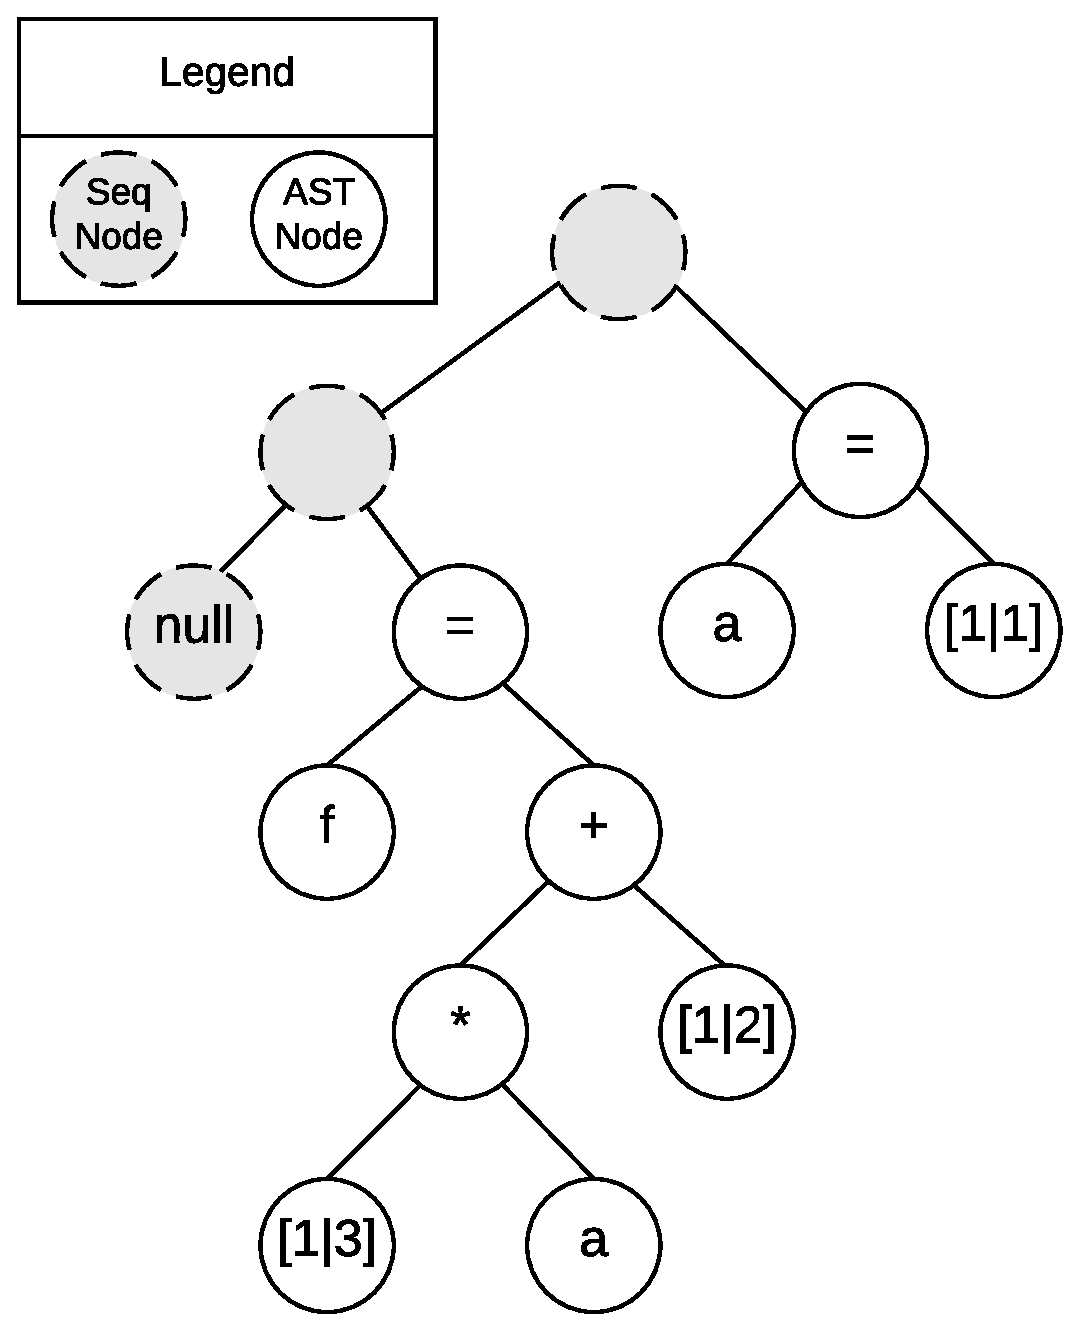
\includegraphics[width=.5\columnwidth]{img/eps/ast.eps}
  \caption{FAC - example of AST.}
  \label{fig:ast}
\end{figure}

\subsection{Error Handling}
We have redefined the standard \verb|yyerror| function provided by bison.
Our \verb|yyerror| implementation is variadic in order to accept any numbers of
arguments. Also, it frees the resources used during parsing before exiting with
the \verb|EXIT_FAILURE| \cite{glibc-online} status code.
